\section*{11.3 \ \ More Problems}

\ 


\begin{enumerate}
\item For any two vectors $\vec{u}$ and $\vec{v}$ use the properties of the dot product to show that
\[
\| \vec{u} \pm \vec{v} \|^2 = \| \vec{u} \|^2 + \| \vec{v} \|^2 \pm 2 (\vec{u} \cdot \vec{v}).
\]

\ 

\item For any two vectors $\vec{u}$ and $\vec{v}$ show that
\[
\| \vec{u} + \vec{v} \|^2 + \| \vec{u} - \vec{v} \|^2 = 2\| \vec{u} \|^2 + 2\| \vec{v} \|^2.
\]
Interpret this as a statement about parallelograms.  \\

\item  Consider two nonzero vectors $\vec{u}$ and $\vec{v}$ and the angle between them $\theta$.  The vectors $\vec{u}$, $\vec{v}$, and $\vec{u} - \vec{v}$ form the triangle as follows.
\begin{center}
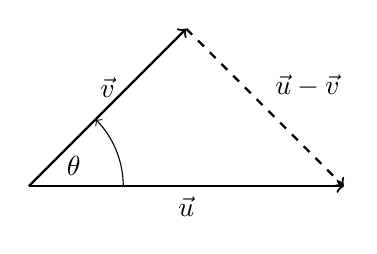
\begin{tikzpicture}[scale=2]
    \draw[thick,->] (0,0) node[anchor=south west]{$\ \ \ \theta$} -- node[anchor=north]{$\vec{u}$} (2,0);
    \draw[thick,->] (0,0) -- node[anchor=south]{$\vec{v}$} (1,1);
    \draw[thick,->, dashed] (1,1) -- node[anchor=south west]{$\vec{u} - \vec{v}$} (2,0);
    \draw[->,thin] (3/5,0) arc [start angle=0, end angle=45, radius=3/5];
\end{tikzpicture}
\end{center}
\begin{enumerate}
\item Use the Law of Cosines to show that
\[
\| \vec{u} - \vec{v} \|^2 = \| \vec{u} \|^2 + \| \vec{v} \|^2 - 2 \| \vec{u} \| \| \vec{v} \| \cos \theta.
\]

\item  Use (a) and the previous problem to conclude the formula 
\[
\vec{u} \cdot \vec{v} = \| \vec{u} \| \| \vec{v} \| \cos \theta.
\] 
\end{enumerate} 

\ 

\item  Suppose we know that $\| \vec{u} \| = 5$, $\| \vec{v} \| = 4$, and the angle between $\vec{u}$ and $\vec{v}$ is $\theta = \pi/3$. Determine the following.
\begin{enumerate}
\item  $\| \vec{u} + \vec{v} \|$.

\item  $\vec{u} \cdot \vec{v}$.

\item  $\| \frac{1}{2} \vec{u} + 3\vec{v} \|$.

\item  $\| \vec{u} - \vec{v} \|$.\\
\end{enumerate}

\item  Show that the two diagonals of a parallelogram intersect in right angles if and only if all four sides of the parallelogram have the same length. \\

\item  Show that for any two vectors $\vec{u}$ and $\vec{v}$ we have
\[
| \vec{u} \cdot \vec{v} | \leq \| \vec{u} \| \ \| \vec{v} \|.
\] 
This is called the \emph{Cauchy-Schwarz inequality}.  \\

\item  Show that for any two vectors $\vec{u}$ and $\vec{v}$ we have
\[
\| \vec{u} + \vec{v} \| \leq \| \vec{u} \| + \| \vec{v} \|.
\] 
This is called the \emph{triangle inequality}.  Explain the name.  \\


\end{enumerate}

